\documentclass[aip,amsmath, reprint, author-year]{revtex4-1}
\usepackage{url}
\usepackage[utf8]{inputenc}
\usepackage{hyperref}
\usepackage{graphicx} % for graphics
%\usepackage{listings} % for code listtings
%\usepackage{color}

%\setcitestyle{round, author-year}

\setcounter{page}{1}

%\bibliographystyle{aipauth4-1.bst}

\begin{document}

\begin{abstract}
A approach to generate Generalized Process Capability Data in order to populate and add functionality to a process capability database.
A description of the concept of generalization, uses and implementation.
\end{abstract}

\title{Concept of using General Process Capability Data}
\author{Andreas Bruun Okholm, s082562\\
Mathias Rask Møller, s082536 }
\affiliation{Technical University of Denmark}
 
\date{\today}
\maketitle

%Introduction

\section{Introduction}

A Process Capability DataBase (PCDB) is a tool for mechanical designers to get information of what is possible to achieve in production. By applying PC information in the design process it is possible to reduces: rework, cost, failure rate, assembly problems and increases product performance.
A in few words a PCDB is a database of variance in features on produced products, different companies has different index system and standard for what to record.

For designer to use a PCDB in the design process, the database has to contain the needed data. The designers themselves does not generate the necessary data and from (Tata) we have learned that the data already recorded in the process control is not necessary the desired data for the mechanical designer. The data desired by the designer are usually the PC of a geometry, material and process in order design for what is achievable in production. The data recoded by process control can be generalized to describe geometries for the process and material instead of specific features on a specific product. 

ISO 286? describes a non-linear function for comparing tolerances on objects of different dimension. This function used to normalize tolerances and display PC independent of size (with in the limits of the function.)  



The purpose of using general process capability data stems from robust design. The idea is to get better at developing a product that are more robust towards variance in production and that way decrease failure rate or cost of changes in production ramp up than otherwise is used to decrease failrate.

 Most inhouse PCDBs have problems with population


In the design process is often a problem to apply tolerances. This aspect of the design phase is often pushed to the very end before production. Features are designed so delicate that in order to meet specification tight tolerances are applied, which can be difficult to produce.
This problem could be solved by looking up the critical tolerance the industry typically can produce to and altering the design for a suitable tolerance.  I that way making tolerance selection a part of the design process.

robust design general

\section{Predicting Process Capability}
The process capability indices has been widely adopted in statistical process control \citep{kane1986process}. Instead of looking at process mean $\mu$ and standard deviation $\sigma$ and their estimates $\hat{\mu}, \hat{\sigma}$ and tolerance upper and lower limits USL, LSL using process capabilities indices transforms these numbers into unit less numbers, which provides a quick overview of how a process is performing.

  


Typically 

\cite{tang1997graphical}

a measurement
a measurement set
std and bias
cpk 
\begin{equation}
C_{pk} = \frac{bias}{3 \, \sigma}
\label{eq:sddj}
\end{equation}


confidence intevals

\section{How much data}


\begin{figure}
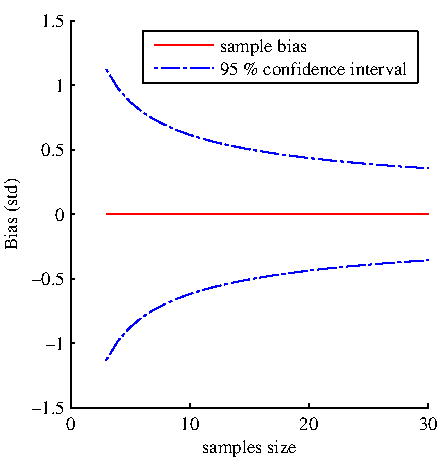
\includegraphics{stats_bias_confidence.pdf}
\caption{\label{fig:std_uncertainty}The uncertainty of the standard deviation estimate is reduced as the number of samples is increased. The increase in accuracy gained per additional decreases with more samples. From the graph we have chosen 12 to be the optimal point for general process capability use.}
\end{figure}



\begin{figure}
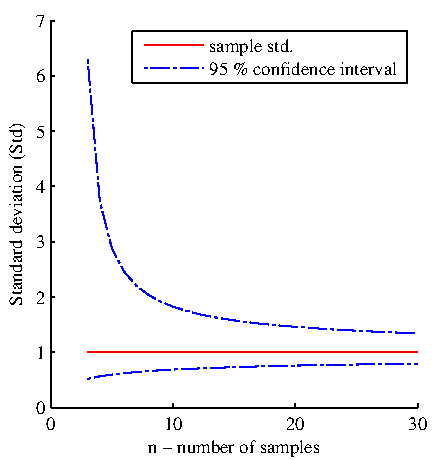
\includegraphics{stats_std_confidence.pdf}
\caption{\label{fig:std_uncertainty}The uncertainty of the standard deviation estimate is reduced as the number of samples is increased. The increase in accuracy gained per additional decreases with more samples. From the graph we have chosen 12 to be the optimal point for general process capability use.}
\end{figure}




sample size  \ref{eq:sddj}




Obtaining Process Capability data is a process of measuring a lot of products.
Products are measured and compared to the nominal size they were produced for, this is called error.

In a production line control measurement are usually done by taking a set of samples to represent the entire population. Each product in the sample set, produces a measurement. From the set of measurements a standard deviation and a mean shift is calculated.

\section{uses}
existance of it-grade
improvement per rework
material selection





By looking at normalized data of the variance of products of the same material and process, it is possible to find a suitable tolerance

\section{implementation}





A cross company platform is suggested to populate the database. The gain is diverse data to be able to compare materials and processes. 

Even relatively big companies in Denmark does not have the resources record 

Since companies tends to be conservative in their production 
By 

The more data the better. The GPC tool's strength is the ability of draw knowledge from actual components of big diversity. Allowing  

In a production company structure consisting of a Production unit, a Mechanical Design unit and a Quality Reassurance unit, the Quality 

A change in the existing system has to be made is .
 



To populate GPC 

Industry secrets
	experience
	
	
active actors and interest groups
	sub suppliers 
	mechanical design consultants
	

difficulties
	Non disclusure agreement
	end-customer
	

\section*{References}
\bibliography{../PCDBmasterBibliography/PCDB_Master_bib.bib}

\end{document}